\section{Overview of our approach}

\begin{figure}
\begin{center}
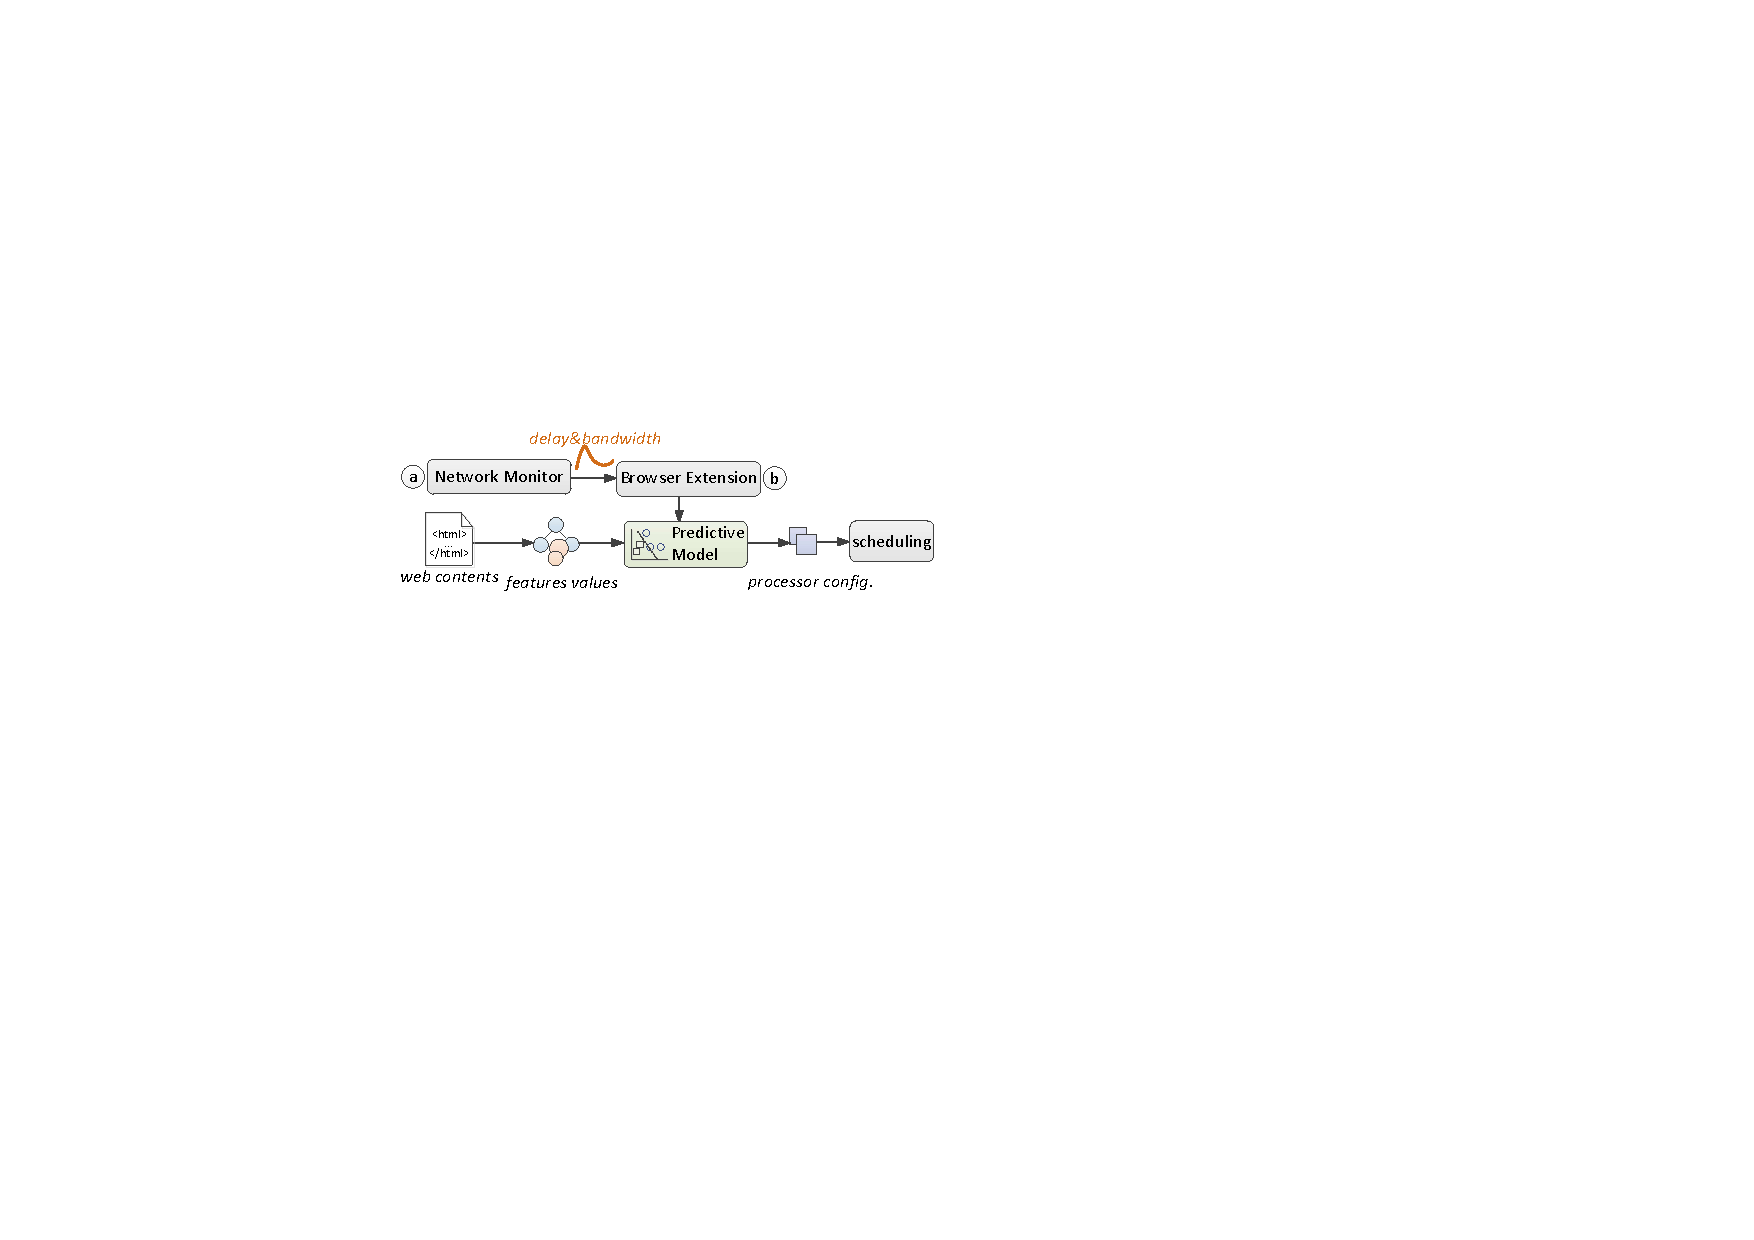
\includegraphics[width=0.5\textwidth]{figure/predictor.pdf}
\end{center}
\caption{Overview of our approach. The network monitor evaluates the network bandwidth and delay to choose a model to predict the
optimum processor configuration. }
\vspace{-4mm}
\label{fig:predictor}
\end{figure}


%Our goal is to develop a better CPU frequency governor to determine which of the multi-core processors to use to run the bowser rendering
%process and at what frequency the heterogeneous processor cores should operate. We target the ARM big.LITTLE heterogeneous multi-core
%architecture as it is now a commonplace on modern mobile devices. Rather than developing a hand-crafted approach that requires expert insight
%into the relative costs and idiosyncrasies of a particular platform and networking environment, we develop an automatic technique that is
%independent of the computing environment.


%We achieve this by employing machine learning to automatically build
%\emph{off-line} models of the platform's behavior, based on prior training data. The learnt models then predicts the best CPU frequency
%decision for any \emph{unseen} webpage in a given networking environment.

Our approach, depicted in Figure~\ref{fig:predictor}, consists of two main components: (i) a network monitor running as an OS service and
(ii) a web browser extension. The network monitor measures the end to end delay and network bandwidths when downloading the webpage. The
web browser extension determines the best processor configuration depending on the network environment and the web contents. Our current
implementation lets the OS to schedule other browser threads such as the input/output and the painting processes. At the heart of our web
browser extension is a set of \emph{off-line} learned predictive models. The predictor takes in a set of numerical values, or
\emph{features values}, which describes the essential characteristics of the webpage. It predicts which core to use to run the rendering
process and at what frequency the heterogeneous processors should operate. The set of features used to describe the webpage is extracted
from the web contents.



%\footnote{Because Chromium for Android currently does not support extensions, we implemented our prototype in Chromium for Linux which
%shares the same code base as the Android Chromium.}
